\documentclass[11pt]{article}

\usepackage[
  textwidth=160mm, textheight=230mm,
  top=32mm, headheight=5pt, headsep=19pt, footskip=32pt
]{geometry}
\usepackage[T1]{fontenc}
\usepackage{mathptmx}
\usepackage{amsmath,amssymb}
\usepackage[round,authoryear]{natbib}
\usepackage{graphicx}
\usepackage{titlesec}
\usepackage[colorlinks=true,linkcolor=blue,citecolor=blue,urlcolor=blue]{hyperref}

\titleformat{\section}
  {\fontsize{11}{13}\selectfont\bfseries\raggedright}{\thesection.}{0.5em}{}
\titlespacing*{\section}{0pt}{26pt plus 4pt minus 2pt}{13pt}
\setlength{\parindent}{10pt}
\setlength{\parskip}{0pt}

\newcommand{\E}{\mathbb{E}}

\title{Empirical Calibration of the Bivariate Kou Model:\\Companion Note}
\author{}
\date{}

\begin{document}
\maketitle

\begin{abstract}
This note accompanies \emph{Optimal Sizing of Leveraged Crypto Long--Short Positions
under Kou Jump-Diffusion via Killed Moments}. It records the penalized empirical
characteristic-function estimator, frequency grid, initialization, and identification
considerations underlying the empirical illustration in the main paper.
\end{abstract}

\section*{Model notation}

We retain the notation of the main paper. For assets $i=1,2$, the free parameter vector is
\[
\theta
=
\bigl((\mu_i,\sigma_i,\lambda_i,p_i,\eta_{i,+},\eta_{i,-})_{i=1,2},\rho\bigr).
\]
Here $\mu_i$ is the expected-price growth exponent, $\sigma_i>0$ is diffusion volatility,
$\lambda_i>0$ is jump intensity, $p_i\in(0,1)$ is the upward-jump probability,
$\eta_{i,+}\in(0,1)$ and $\eta_{i,-}>0$ are the mean upward and downward jump sizes, and
$|\rho|<1$ is Brownian correlation. The jump characteristic function and price-jump
compensator are
\[
\varphi_{J_i}(u)
=
\frac{p_i}{1-iu\eta_{i,+}}+\frac{1-p_i}{1+iu\eta_{i,-}},
\qquad
\chi_i
=
\frac{p_i}{1-\eta_{i,+}}+\frac{1-p_i}{1+\eta_{i,-}}-1,
\]
and the derived log-price drift is
$\mu_i^X=\mu_i-\tfrac12\sigma_i^2-\lambda_i\chi_i$. Thus
\[
\Psi_\theta(u,v)
=
i(\mu_1^Xu+\mu_2^Xv)
-\frac12\bigl(\sigma_1^2u^2+\sigma_2^2v^2+2\rho\sigma_1\sigma_2uv\bigr)
+\lambda_1\bigl(\varphi_{J_1}(u)-1\bigr)
+\lambda_2\bigl(\varphi_{J_2}(v)-1\bigr).
\]
The liquidation-driving log-price spread is $Z=X_1-X_2$. If moments through order $K$
are required, the admissibility restriction is $K\eta_{i,+}<1$ for $i=1,2$.

\section{Penalized ECF estimator}\label{sec:ecf-estimator}

The closed-form Lévy--Khintchine exponent $\Psi_\theta(u,v)$ gives the
model-implied characteristic function
\begin{equation}\label{eq:model-cf}
\phi_\theta(u,v;\Delta)
=
\exp\!\bigl(\Delta\,\Psi_\theta(u,v)\bigr),
\end{equation}
where $\Delta$ is the observation interval.
Given $N$ observed bivariate log-return pairs $(r_{1,n},r_{2,n})_{n=1}^N$,
the empirical characteristic function is
\begin{equation}\label{eq:ecf}
\widehat{\phi}_N(u,v)
=
\frac{1}{N}\sum_{n=1}^N
\exp\!\bigl(i(u\,r_{1,n}+v\,r_{2,n})\bigr).
\end{equation}
The ECF component of the estimator is the normalized weighted squared distance
between \eqref{eq:ecf} and \eqref{eq:model-cf} over a discrete frequency grid
$\mathcal{G}$:
\begin{equation}\label{eq:ecf-objective}
Q_N^{\mathrm{ECF}}(\theta)
=
\frac{\displaystyle\sum_{(u,v)\in\mathcal{G}}w(u,v)
\,\bigl|\widehat{\phi}_N(u,v)-\phi_\theta(u,v;\Delta)\bigr|^2}
{\displaystyle\sum_{(u,v)\in\mathcal{G}}w(u,v)}.
\end{equation}
Because finite high-frequency samples leave a pronounced intensity--jump-size ridge, the
reported calibration uses two transparent soft anchoring terms:
\begin{equation}\label{eq:ecf-penalized-objective}
\begin{aligned}
\widehat{\theta}
&=\arg\min_{\theta\in\Theta}\mathcal{Q}_N(\theta),\\
\mathcal{Q}_N(\theta)
&=Q_N^{\mathrm{ECF}}(\theta)
+\omega_\lambda\sum_{i=1}^{2}(\log\lambda_i-\log\widetilde\lambda_i)^2\\
&\quad+\omega_\eta\sum_{i=1}^{2}\sum_{s\in\{+,-\}}
(\log\eta_{i,s}-\log\widetilde\eta_{i,s})^2.
\end{aligned}
\end{equation}
Here $\widetilde\lambda_i$ is the variance/fourth-cumulant initializer and
$\widetilde\eta_{i,s}$ is the peak-over-threshold (POT) mean-excess initializer described
below. The application uses $(\omega_\lambda,\omega_\eta)=(0.05,0.02)$. These are soft
penalties, not equality restrictions; setting both weights to zero recovers pure ECF
matching.
This is the empirical-characteristic-function approach of
\citet{Singleton2001}, which is particularly natural for affine and
Lévy-based asset-pricing models whose characteristic functions are known in
closed form.
\citet{FeuervergerMcDunnough1981} establish that ECF estimators over a
rich grid can attain maximum-likelihood efficiency.
The procedure avoids evaluating the bivariate transition density, which would
require a two-dimensional numerical Fourier inversion inside every optimizer
call.
For background on DEJD likelihood estimation in the univariate case
see \citet{RamezaniZeng2007}.

\section{Frequency grid}\label{sec:ecf-grid}

The parameter vector $\theta$ has the $13$ free components stated above.
Raw return magnitudes depend on the sampling interval, so fixed raw Fourier frequencies
are poorly portable. Let $s_1$, $s_2$, and $s_Z$ be IQR-based robust scales,
$s=\max\{(q_{0.75}-q_{0.25})/1.349,10^{-8}\}$, for $r_1$, $r_2$, and $r_1-r_2$. Dimensionless base
frequencies are mapped to raw frequencies by division by the corresponding scale. The
grid contains the following groups, with every point accompanied by its conjugate
$(-u,-v)$:
\begin{itemize}
  \item marginal points $(a/s_1,0)$ and $(0,a/s_2)$ for
    $a\in\mathcal{A}_{\mathrm{marg}}$;
  \item same-sign and mixed-sign joint points
    $(a/s_1,b/s_2)$ and $(a/s_1,-b/s_2)$ for
    $a,b\in\mathcal{A}_{\mathrm{joint}}$, which are informative about $\rho$;
  \item spread points $(a/s_Z,-a/s_Z)$ for $a\in\mathcal{A}_Z$, which directly
    match the log-ratio process governing liquidation; and
  \item high-base marginal and spread points for $a\in\mathcal{A}_{\mathrm{tail}}$,
    included to retain information about jump-tail shape.
\end{itemize}
The dimensionless base nodes are
\begin{align*}
\mathcal{A}_{\mathrm{marg}}&=\{0.1,0.2,0.5,0.75,1,1.5,2,3,5,7.5,10\},\\
\mathcal{A}_{\mathrm{joint}}&=\{0.25,0.5,1,2,3,5\},\\
\mathcal{A}_{Z}&=\{0.1,0.2,0.5,0.75,1,1.5,2,3,5\},\\
\mathcal{A}_{\mathrm{tail}}&=\{8,12,16,20,25\}.
\end{align*}
Points whose absolute raw coordinate exceeds $5{,}000$ are discarded to avoid numerical
aliasing. Including conjugate pairs, the unfiltered construction has 236 frequency
evaluations; this cap leaves 234 for the application sample. Weights depend on dimensionless
rather than raw frequency:
\[
w(a,b)=\exp\{-0.02(a^2+b^2)\}.
\]
The ordinary spread group receives an additional factor of two. Thus the criterion
emphasizes the barrier-driving ratio without making the choice of observation interval
determine the effective frequency weights.

\section{Reparameterisation and initialisation}\label{sec:ecf-init}

\paragraph{Unconstrained reparameterisation.}
The parameter constraints stated above are enforced automatically via the
change of variables
\begin{equation}\label{eq:reparam}
\sigma_i=e^{a_i},\quad
\lambda_i=e^{b_i},\quad
p_i=\mathrm{sigmoid}(c_i),\quad
\eta_{i,+}=\eta_{i,+}^{\max}\mathrm{sigmoid}(d_i),\quad
\eta_{i,-}=e^{e_i},\quad
\rho=\tanh(f),
\end{equation}
where sigmoid$(x)=(1+e^{-x})^{-1}$.
The unconstrained vector $\tau=({\mu_1,a_1,b_1,c_1,d_1,e_1,\mu_2,\ldots,f})$
is optimized with box bounds in this transformed space. For both assets the code uses
a scaled sigmoid with
\[
\eta_{i,+}^{\max}\le (1-\varepsilon)/K,
\qquad i=1,2,
\]
so that $K\eta_{i,+}<1$ is enforced for $i=1,2$, ensuring finiteness of the
exponential moments used through order $K$.

\paragraph{Threshold initialiser.}
The characteristic-function objective is non-linear and non-convex,
so the optimisation is initialised by a threshold-based decomposition
following the logic of \citet{Mancini2009} for discretely observed
jump-diffusions.
Let $m_i=\mathrm{median}(r_{i,n})$ and let $s_i$ be the IQR robust scale.
For a frequency-aware threshold constant $c\in[3,5]$, define candidate
jump observations
\[
\mathcal{J}_i=\{n:|r_{i,n}-m_i|>c\,s_i\},
\qquad
\mathcal{C}_i=\{1,\ldots,N\}\setminus\mathcal{J}_i.
\]
Initial volatility and correlation values use the continuous subset
$\mathcal{C}_i$, while the jump-size means are anchored by peak-over-threshold
excess means and the intensities are corrected by a variance/fourth-cumulant
estimate.  Schematically:
\begin{align*}
p_i^{(0)}&=\frac{|\mathcal{J}_{i,+}|}{|\mathcal{J}_i|}
  \quad\text{clamped to the admissible probability range},\\
\eta_{i,+}^{(0)},\,\eta_{i,-}^{(0)}&=\text{POT mean-excess estimates},\\
\lambda_i^{(0)}&=\text{two-moment estimate from variance and fourth cumulant},\\
\sigma_i^{(0)}&=\mathrm{sd}(r_{i,n}:\,n\in\mathcal{C}_i)/\sqrt{\Delta},
&
\rho^{(0)}&=\mathrm{corr}(r_1,r_2)_{n\in\mathcal{C}_1\cap\mathcal{C}_2}.
\end{align*}
The initializer first estimates the annualized log-process drift with a damped
mean-jump correction,
\[
\mu_i^{X,(0)}=\bar{r}_i/\Delta
-0.25\,\lambda_i^{(0)}
\left[p_i^{(0)}\eta_{i,+}^{(0)}-(1-p_i^{(0)})\eta_{i,-}^{(0)}\right],
\]
then stores the result in the paper's price-growth convention,
\[
\mu_i^{(0)}=\operatorname{clip}_{[\mu_{\min},\mu_{\max}]}
\!\left(\mu_i^{X,(0)}+\tfrac12(\sigma_i^{(0)})^2
+\lambda_i^{(0)}\chi_i^{(0)}\right).
\]
The threshold filter is not the final estimator.
It is a warm start that places the optimizer in a sensible region of
parameter space; see the remark in \citet{Mancini2009}.

\paragraph{Multi-start cloud.}
Because $\mathcal{Q}_N(\tau)$ may have local minima, the optimizer is run from a
structured cloud. It contains the unperturbed initializer and six deterministic
intensity--size ridge starts with
\[
\lambda_i\mapsto c\lambda_i,\qquad
\eta_{i,\pm}\mapsto\eta_{i,\pm}/\sqrt{c},qquad
c\in\{0.1,0.25,0.5,2,4,8\}.
\]
Remaining starts cycle through four high-jump/high-diffusion scenarios and add bounded
random perturbations to scale, probability, correlation, and drift parameters. The
application calibration uses 30 starts (the library default is 20) and returns the bounded
L-BFGS-B minimizer with the lowest penalized objective.

\section{Identifiability and model-comparison protocol}\label{sec:ecf-ident}

The penalized criterion $\mathcal{Q}_N(\theta)$ is non-convex.
Jump-diffusion models possess approximate ridges along directions that
preserve the compound-Poisson variance contribution
$\lambda_i\E[J_i^2]=2\lambda_i(p_i\eta_{i,+}^2+(1-p_i)\eta_{i,-}^2)$
\citep{RamezaniZeng2007}.
The diffusion volatilities $\sigma_i$ and the Brownian correlation $\rho$
are generally better identified from short samples than jump-size and intensity
parameters, which carry larger finite-sample uncertainty unless the observation
window contains many jump events. Because $\lambda_i$ is annualized, a one-year
window contains $\lambda_i$ jumps in expectation, irrespective of whether prices
are sampled hourly or daily. Finer sampling can make individual jumps easier to
separate from aggregated returns, but it does not multiply the underlying annual
Poisson count.

For descriptive fit comparisons on a common grid, compare the unpenalized component
$Q_N^{\mathrm{ECF}}(\widehat\theta)$ across nested models (GBM, Merton, bivariate Kou),
rather than the penalized values $\mathcal{Q}_N(\widehat\theta)$ whose anchors differ.
Such comparisons should be accompanied by liquidation-relevant diagnostics:
empirical versus model $Z$-tail quantiles, empirical versus model
barrier-crossing frequencies, and simulated versus observed drawdowns of $Z$.
These are more directly informative for the sizing application than
standard likelihood-based criteria.
The present empirical illustration does not carry out a formal GBM--Merton--Kou selection
exercise. Its point calibration and sizing results remain conditional on the selected Kou
model and stated empirical choices; they are not evidence of model dominance or
parameter-robust recommendations.

The repository's calibration package contains the implementation. The
synthetic calibration job shows parameter recovery and produces
Figure~\ref{fig:ecf-fit}.

\clearpage
\begin{figure}[!ht]
\centering
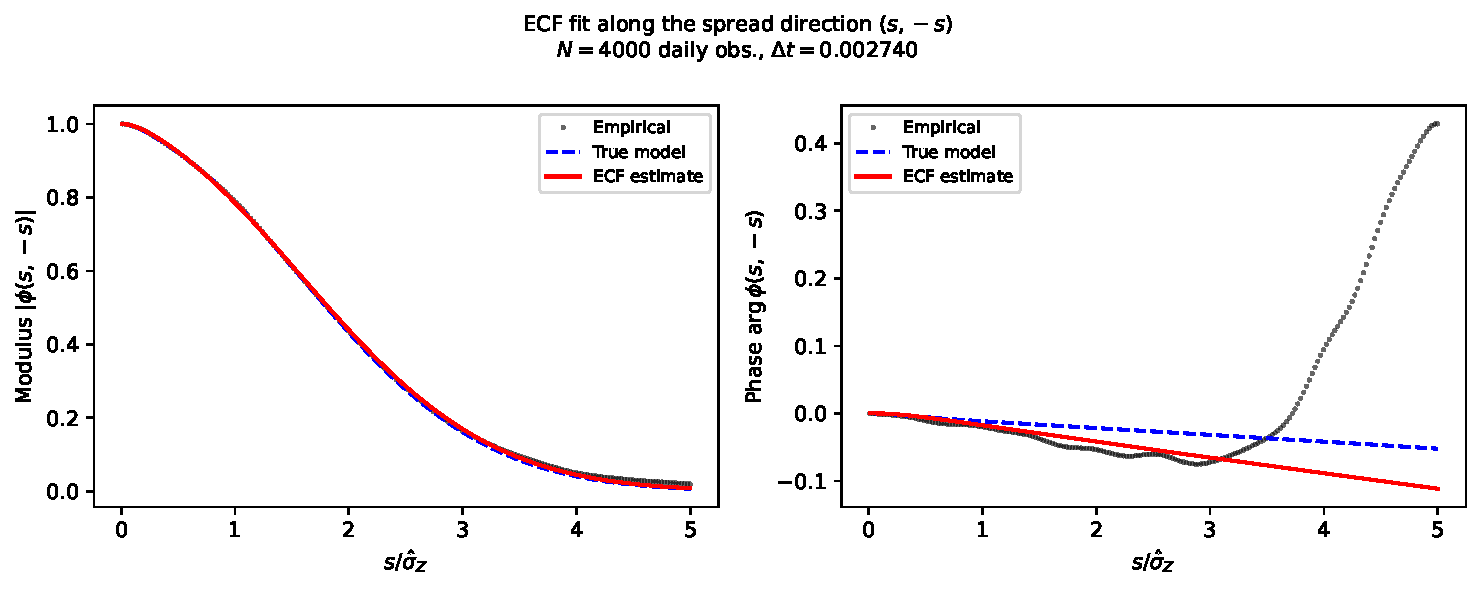
\includegraphics[width=0.85\linewidth]{fig_ecf_fit.pdf}
\caption{ECF fit along the spread direction $(s,-s)$ for $N=4{,}000$
synthetic daily log-return observations.
Left: modulus $|\phi(s,-s)|$; right: phase $\arg\phi(s,-s)$.
Dots: empirical CF $\widehat\phi_N$; dashed: true model CF;
solid red: ECF estimate.
The close agreement in modulus and phase documents the fit along the
liquidation-relevant spread direction; this plot alone does not assess every component of
the full-grid criterion.
Script \texttt{jobs/calibrate\_kou.py}.}
\label{fig:ecf-fit}
\end{figure}

\bibliographystyle{abbrvnat}
\bibliography{finance}

\end{document}
